%%%%%%%%%%%%%%%%%%%%%%%%%%%%%%%%%%%%%%%%%
% Masters/Doctoral Thesis 
% LaTeX Template
% Version 1.43 (17/5/14)
%
% This template has been downloaded from:
% http://www.LaTeXTemplates.com
%
% Original authors:
% Steven Gunn 
% http://users.ecs.soton.ac.uk/srg/softwaretools/document/templates/
% and
% Sunil Patel
% http://www.sunilpatel.co.uk/thesis-template/
%
% License:
% CC BY-NC-SA 3.0 (http://creativecommons.org/licenses/by-nc-sa/3.0/)
%
% Note:
% Make sure to edit document variables in the Thesis.cls file
%
%%%%%%%%%%%%%%%%%%%%%%%%%%%%%%%%%%%%%%%%%

%----------------------------------------------------------------------------------------
%	PACKAGES AND OTHER DOCUMENT CONFIGURATIONS
%----------------------------------------------------------------------------------------

\documentclass[11pt, oneside]{Thesis} % The default font size and one-sided printing (no margin offsets)

\graphicspath{{Pictures/}} % Specifies the directory where pictures are stored

\usepackage{epigraph}
\usepackage[square, numbers, comma, sort&compress]{natbib} % Use the natbib reference package - read up on this to edit the reference style; if you want text (e.g. Smith et al., 2012) for the in-text references (instead of numbers), remove 'numbers' 
\hypersetup{urlcolor=blue, colorlinks=true} % Colors hyperlinks in blue - change to black if annoying
\title{\ttitle} % Defines the thesis title - don't touch this


\begin{document}

\frontmatter % Use roman page numbering style (i, ii, iii, iv...) for the pre-content pages

\setstretch{1.3} % Line spacing of 1.3

% Define the page headers using the FancyHdr package and set up for one-sided printing
\fancyhead{} % Clears all page headers and footers
\rhead{\thepage} % Sets the right side header to show the page number
\lhead{} % Clears the left side page header

\pagestyle{fancy} % Finally, use the "fancy" page style to implement the FancyHdr headers

\newcommand{\HRule}{\rule{\linewidth}{0.5mm}} % New command to make the lines in the title page
\newcommand{\uniname}{Universidad del Norte}

% PDF meta-data
\hypersetup{pdftitle={\ttitle}}
\hypersetup{pdfsubject=\subjectname}
\hypersetup{pdfauthor=\authornames}
\hypersetup{pdfkeywords=\keywordnames}

%----------------------------------------------------------------------------------------
%	TITLE PAGE
%----------------------------------------------------------------------------------------

\begin{titlepage}
\begin{center}

\textsc{\LARGE \uniname}\\[1.5cm] % University name
\textsc{\Large Master Thesis}\\[0.5cm] % Thesis type

\HRule \\[0.4cm] % Horizontal line
{\huge \bfseries Visual Object Tracking applying ensemble of multiple trackers}\\[0.4cm] % Thesis title
\HRule \\[1.5cm] % Horizontal line
 
\begin{minipage}{0.4\textwidth}
\begin{flushleft} \large
\emph{Author:}\\
Jorge Martinez Gomez % Author name - remove the \href bracket to remove the link
\end{flushleft}
\end{minipage}
\begin{minipage}{0.4\textwidth}
\begin{flushright} \large
\emph{Supervisor:} \\
\href{http://niebles.net}{Juan Carlos Niebles} % Supervisor name - remove the \href bracket to remove the link  
\end{flushright}
\end{minipage}\\[3cm]
 
\large \textit{A thesis submitted in fulfilment of the requirements\\ for the degree of Master of Science}\\[0.3cm] % University requirement text
\textit{in the}\\[0.4cm]
Computer Vision Research Group\\Electrical and Electronics engineering department\\[2cm] % Research group name and department name
 
{\large \today}\\[4cm] % Date
%\includegraphics{Logo} % University/department logo - uncomment to place it
 
\vfill
\end{center}

\end{titlepage}

%----------------------------------------------------------------------------------------
%	DECLARATION PAGE
%	Your institution may give you a different text to place here
%----------------------------------------------------------------------------------------

\Declaration{

\addtocontents{toc}{\vspace{1em}} % Add a gap in the Contents, for aesthetics

I, \authornames, declare that this thesis titled, '\ttitle' and the work presented in it are my own. I confirm that:

\begin{itemize} 
\item[\tiny{$\blacksquare$}] This work was done wholly or mainly while in candidature for a research degree at this University.
\item[\tiny{$\blacksquare$}] Where any part of this thesis has previously been submitted for a degree or any other qualification at this University or any other institution, this has been clearly stated.
\item[\tiny{$\blacksquare$}] Where I have consulted the published work of others, this is always clearly attributed.
\item[\tiny{$\blacksquare$}] Where I have quoted from the work of others, the source is always given. With the exception of such quotations, this thesis is entirely my own work.
\item[\tiny{$\blacksquare$}] I have acknowledged all main sources of help.
\item[\tiny{$\blacksquare$}] lelele
\item[\tiny{$\blacksquare$}] Where the thesis is based on work done by myself jointly with others, I have made clear exactly what was done by others and what I have contributed myself.\\
\end{itemize}
 
Signed:\\
\rule[1em]{25em}{0.5pt} % This prints a line for the signature
 
Date:\\
\rule[1em]{25em}{0.5pt} % This prints a line to write the date
}

\clearpage % Start a new page

%----------------------------------------------------------------------------------------
%	QUOTATION PAGE
%----------------------------------------------------------------------------------------

\pagestyle{empty} % No headers or footers for the following pages

\null\vfill % Add some space to move the quote down the page a bit

\textit{``Thanks to my solid academic training, today I can write hundreds of words on virtually any topic without possessing a shred of information, which is how I got a good job in journalism."}

\begin{flushright}
Dave Barry
\end{flushright}

\vfill\vfill\vfill\vfill\vfill\vfill\null % Add some space at the bottom to position the quote just right

\clearpage % Start a new page

%----------------------------------------------------------------------------------------
%	ABSTRACT PAGE
%----------------------------------------------------------------------------------------

\addtotoc{Abstract} % Add the "Abstract" page entry to the Contents

\abstract{\addtocontents{toc}{\vspace{1em}} % Add a gap in the Contents, for aesthetics

The Thesis Abstract is written here (and usually kept to just this page). The page is kept centered vertically so can expand into the blank space above the title too\ldots
}

\clearpage % Start a new page

%----------------------------------------------------------------------------------------
%	ACKNOWLEDGEMENTS
%----------------------------------------------------------------------------------------

\setstretch{1.3} % Reset the line-spacing to 1.3 for body text (if it has changed)

\acknowledgements{\addtocontents{toc}{\vspace{1em}} % Add a gap in the Contents, for aesthetics
%\epigraph{Not enough people in this world, I think, carry a cosmic perspective with them. It could be life-changing.}{Neil deGrasse Tyson}
%\epigraph{TheBigBangTheory: When geeky scientists can be main characters in a hit primetime series, you know there's hope for the world.}{Neil deGrasse Tyson}

\epigraph{Not enough people do things that leave others to wonder.  RT @BrianMendicino: Wondering why @neiltyson is watching Glee.}{Neil deGrasse Tyson}

The acknowledgements and the people to thank go here, don't forget to include your project advisor\ldots
}
\clearpage % Start a new page

%----------------------------------------------------------------------------------------
%	LIST OF CONTENTS/FIGURES/TABLES PAGES
%----------------------------------------------------------------------------------------

\pagestyle{fancy} % The page style headers have been "empty" all this time, now use the "fancy" headers as defined before to bring them back

\lhead{\emph{Contents}} % Set the left side page header to "Contents"
\tableofcontents % Write out the Table of Contents

\lhead{\emph{List of Figures}} % Set the left side page header to "List of Figures"
\listoffigures % Write out the List of Figures

\lhead{\emph{List of Tables}} % Set the left side page header to "List of Tables"
\listoftables % Write out the List of Tables

%----------------------------------------------------------------------------------------
%	ABBREVIATIONS
%----------------------------------------------------------------------------------------

\clearpage % Start a new page

\setstretch{1.5} % Set the line spacing to 1.5, this makes the following tables easier to read

\lhead{\emph{Abbreviations}} % Set the left side page header to "Abbreviations"
\listofsymbols{ll} % Include a list of Abbreviations (a table of two columns)
{
\textbf{LAH} & \textbf{L}ist \textbf{A}bbreviations \textbf{H}ere \\
%\textbf{Acronym} & \textbf{W}hat (it) \textbf{S}tands \textbf{F}or \\
}

%----------------------------------------------------------------------------------------
%	PHYSICAL CONSTANTS/OTHER DEFINITIONS
%----------------------------------------------------------------------------------------

\clearpage % Start a new page

\lhead{\emph{Physical Constants}} % Set the left side page header to "Physical Constants"

\listofconstants{lrcl} % Include a list of Physical Constants (a four column table)
{
Speed of Light & $c$ & $=$ & $2.997\ 924\ 58\times10^{8}\ \mbox{ms}^{-\mbox{s}}$ (exact)\\
% Constant Name & Symbol & = & Constant Value (with units) \\
}

%----------------------------------------------------------------------------------------
%	SYMBOLS
%----------------------------------------------------------------------------------------

\clearpage % Start a new page

\lhead{\emph{Symbols}} % Set the left side page header to "Symbols"

\listofnomenclature{lll} % Include a list of Symbols (a three column table)
{
$a$ & distance & m \\
$P$ & power & W (Js$^{-1}$) \\
% Symbol & Name & Unit \\

& & \\ % Gap to separate the Roman symbols from the Greek

$\omega$ & angular frequency & rads$^{-1}$ \\
% Symbol & Name & Unit \\
}

%----------------------------------------------------------------------------------------
%	DEDICATION
%----------------------------------------------------------------------------------------

\setstretch{1.3} % Return the line spacing back to 1.3

\pagestyle{empty} % Page style needs to be empty for this page

\dedicatory{For/Dedicated to/To my\ldots} % Dedication text

\addtocontents{toc}{\vspace{2em}} % Add a gap in the Contents, for aesthetics

%----------------------------------------------------------------------------------------
%	THESIS CONTENT - CHAPTERS
%----------------------------------------------------------------------------------------

\mainmatter % Begin numeric (1,2,3...) page numbering

\pagestyle{fancy} % Return the page headers back to the "fancy" style

% Include the chapters of the thesis as separate files from the Chapters folder
% Uncomment the lines as you write the chapters


\input{Chapters/introduction}
% Chapter Template

\chapter{Moving Object Detection Approaches, Challenges, Datasets and Object Tracking} % Main chapter title

\label{chapter2} % Change X to a consecutive number; for referencing this chapter elsewhere, use \ref{ChapterX}

\lhead{Chapter 2. \emph{Moving Object Detection Approaches, Challenges and Object Tracking}} 

An object can be considered simply as nothing but an entity of interest used for further analysis. These elements can be represented by their shape \textbf{Cite here} or appearance \textbf{cite color histograms, etc.}. In order to track objects, selecting the right features plays a critical role. In general, the most important property of a visual feature is its uniqueness so that could be easily distinguished from other objects. Mostly features are chosen manually by the user depending on the application domain. this problem of automatic feature selection has receibed significant attention in the pattern recognition community. The most common visual features selections are color, edges, displacement vectors and textures.

Among all features, color is the one of the most widely used feature for tracking. However, color features are sensity to illumination variation. To tackle this problem, in scenarios where this effect is inevitable, other features are incorporated to model object appearance.

\section{Moving Object Detection}

In a video, there are two sources of information that can be used for object detection and tracking: Visual features (color, texture and shape) and motion information. Robust approaches suggest that combining the statistical analysis of visual features and temporal analysis of motion information. Moving object detection targets the extraction of moving objects that are of interest in sequences (e.g. people and vehicles).

A large number of methodologies have been proposed for object tracking, focusing on the task of object detection first. Most of them apply combinations and intersections among different methodologies, making it very difficult to create a uniform classification of existing approaches. This section classifies different approaches available for object detection from videos.

\subsection{Background Substraction}

Background subtraction is a commonly used technique for object segmentation in static scenarios \cite{McIvor2000}. This task consist in detecting moving regions by subtracting the current image pixel-by-pixel from a reference background image. The pixels above some threshold are classified as foreground (belongs to an object). The background image is created averaging images over time in an intiialization period, and is updated with new images to adapt to dynamic scene changes. Also, the foreground map is followed by morphological operations such as closing and erosion (elimination of small-sized blobs).

Although background subtraction techniques extracts well most of the relevant pixels, this method is sensitive to changes when some background and foreground pixels have similar value.

\begin{figure}[h!]
	\centering
		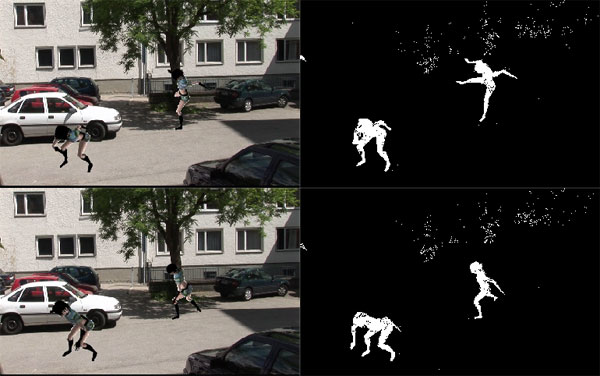
\includegraphics[width=0.7\linewidth]{Figures/bg_sub.jpg}
	\caption{Object detection using Gaussian Mixture Models for background subtraction \cite{Pham2010}. foreground pixels are drawn in white.}
	\label{fig::bg_sub}
\end{figure}

\subsection{Temporal differencing}

In temporal differencing, objects are detected by taking pixel-by-pixel difference of consecutive frames (generally two or three) in a video sequence. This method is most common for moving object detection in scenarios where camera is moving. Unlike static camera scenarios, the background is changing in time for moving camera (not appropiate to create a background model). Alternatively, the moving object is detected by taking the difference between frames $t - 1$ and $t$.

This method is highly adaptive to dynamic changes in the scene as most recent frames are involved in the process. However, it fails detecting small regions as moving objects (ghost regions). Detection will not be correct also, for objects that preserve uniform regions (static objects).

A two-frame differencing method is presented in \cite{Lipton1998a}, where the pixels that satisfy the following equation are marked as foreground.\\
\centerline{$|I_t(x,y), I_{t-1}(x,y)|>Th$}

Other methods were developed in order to overcome drastic changes of two frame differencing in some cases. For instance, a three-frame differencing method \cite{Wang2003} and a hybrid method that combines three-frame differencing with an adaptive background subtraction model \cite{Collins2000}.

\subsection{Statistical Approaches}

Statistical characteristics of pixels have been used, in order to overcome shortcomings between frames of basic background subtraction methods. The approaches consist in keeping and updating pixels statistics that belong to the background model. Foreground pixels are identified by comparing each pixel's statistics with that of the background model. These methods are becoming more popular due to its reliability in scenes that contain noise, illumination changes and shadows. For instance, some approaches apply Hidden Markov Models (HMM). These methods \cite{Stenger2001,Rittscher2000} represent the intensity variation of a pixel in an image sequence as discrete states

The statistical method proposed in \cite{Pham2010} describes and adaptive background model for real-time tracking. Every pixel is modeled by a mixture of Gaussians which are udpated online using incoming image data. Then, the Gaussians distributions of the mixture model for each pixel is evaluated in order to detect whether a pixel belongs to foreground and background.

\subsection{Point detectors}

Point detectors are used to find interesting points in objects which have an expressive texture in their respective localities. An interest point should have invariance to changes in illumination and camera viewpoint. One important detector uses optical flow approach \cite{Shi1994}. These methods make use of the flow vectors of moving objects over time to detect moving blobs in an image. In this approach the apparent velocity and direction of every pixel in the frame must be computed. Some other methods are SIFT \cite{Lowe2004b} and Harris \cite{Harris1988} corners detectors.

\begin{figure}[h!!]
\centering
{
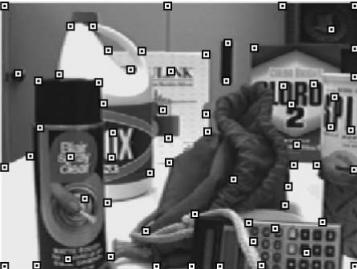
\includegraphics[width=0.32\linewidth]{Figures/points/harris.png}
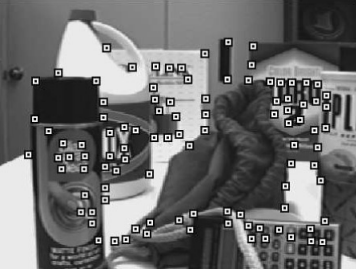
\includegraphics[width=0.32\linewidth]{Figures/points/klt.png}
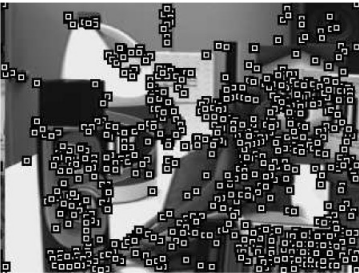
\includegraphics[width=0.32\linewidth]{Figures/points/sift.png}
}	
\end{figure}

\section{Challenges}

Object detection and tracking is still an open research problem in computer vision. A robust, accurate and high performance approach is still a great challenge. The level of difficulty depends on how the object of interest is defined in terms of features. For instance, Using color as object representation method, it is not difficult to identify all pixels with same color as the object. However, there is always a probability of existence a background region with same color information (background clutter). In addition, illumination changes in the scene does not guarantee that the pixel values of an object will be the same in all frames. These variabilities or challenges which are random in object tracking causes wrong object tracking, and are listed below.

\begin{itemize}
\item \textbf{Illumination Variation (IV):} It is desirable that background model adapts to gradual changes of the appearance of the environment.
\item \textbf{Scale Variation (SV):} Ratio between initial object size and current object size differs.
\item \textbf{Occlusion (OC):} Partially or full, occlusion affects the process of computing the background frame. In real life situations, occlusion can occur anytime the object of interest passes behind another object with respect to a camera.
\item \textbf{Dynamic background:} Some scenery regions contain movement, but should be still remain as background, acoording to their relevance. Such movement can be periodical or irregular, causing blurring (motion blur - MB), e.g. traffic lights, waving trees).
\item \textbf{Out of view (OV): } Some portion o the target leaves the view.
\item \textbf{Background clutter (BC):} As stated before, this challenge makes the segmentation task difficult. It is hard to create ans separate background model from moving foreground objects.
\item \textbf{Fast Motion (FM):} The speed of a moving object plays an important role in its detection and track. If an object is moving too slow, the temporal differencing methods fails to detect object, because it preserves uniform region between frames. In the other case, fast moving object leaves ghost regions in a detected foreground model.
\item \textbf{Object rotation and deformation (DEF):} Since natural objects move freely, they can appear slightly or completely transformed. Such rotations, in (IPR) or out (OPR) of plane on the images affect object tracking considerably.
\item \textbf{Low Resolution (LR):} Number of pixels inside the object bounding box is less than 400.
\end{itemize}

\section{Tracking Datasets}

In computer vision, a \textit{dataset} could be defined as a collection of images or video sequences used for testing algorithms. The amount of data and characteristics presented in the list, depend on the field that is studied. For instance, in scene recognition, a dataset contains images of landscapes or outdoor environments. Generally, this collection is shared between researchers and plays an important role in comparison and evaluation of state-of-the-art approaches.

The Surveillance Performance Evaluation Initiative (SPEVI) can be used for evaluating algorithms for surveillance-related applications. The first dataset contains 5 sequences applied to single person/face detection and tracking. The second dataset applies for multiple person/face detection and tracking. The sequences contain four targets occluding each other repeatedly. ETISEO dataset contains indoor and outdoor scenes, such as corridors, buildings entries, etc. This dataset can be used for surveillance applications.

PETS dataset became a surveillance project whose challenging scenarios are focused only on high level applications of this field. Some issues, like illumination or scale changes are not considered in these videos. Most of the sequences are used for person/vehicle tracking in outdoor environments(subway stations, building entrances). CAVIAR is a dataset used generally for situation recognition systems. However, sequences can be applied for tracking evaluation methods. Includes videos of people walking alone, meeting other people, entering and exiting shops.

The VIdeo Surveillance Online Repository (VISOR) database covers a wide range of scenarios and situations, including videos for human action recognition, outdoor videos for face detection, indoor videos for people tracking with occlusions, vehicles detection and surveillance. The VIdeo Surveillance Online Repository, includes several sequences for two separate tasks: First, an abandoned baggage scenario and second, a parked vehicle scenario.

In generic visual tracking, a dataset is a collection of videos that contains and object moving in some scenario. The sequences vary in length from hundreds of frames to thousands. Diverse object types are used. Different scene settings (indoor or outdoor, static or moving camera). Also different challenges, such as object occlusions or illumination conditions are presented. Most commonly used tracking benchmarks are summarized in table \ref{table:datasets}.  Recently, the authors in \cite{Wu2013b} released a benchmark containing 50 most commonly used sequences from some datasets mentioned \ref{table:datasets}, to facilitate fair performance evaluation. Also for better evaluation and analysis of strengths and weakness of tracking approaches. They classified sequences, considering a object tracking challenge, as a category, constructing several subsets to report specific challenging conditions. Some attributes occur more frequently, and some sequences are annotated with several attributes.

\begin{table}[h!]
\centering
\begin{tabular}{|ll|}
\hline
Name/Author/Paper & Sequences \\
Babenko           & 3         \\
Bobot             & 12        \\
Cehovin           & 5         \\
Ellis IJCV2011    & 3         \\
Godec             & 7         \\
Kalal             & 10        \\
Kwon              & 4         \\
Kwon VTD          & 11        \\
PROST             & 4         \\
Ross              & 4         \\
Thang             & 4         \\
Wang              & 4         \\
\hline
\end{tabular}
\caption{Popular object tracking datasets}
\label{table:datasets}
\end{table}

\section{Object Tracking}

The goal of an object tracker is to generate an object path over time. This trajectory consists of the object position over time in every frame of the video. The tracker may provide complete region in the image that is occupied by the object at every time instant. Certainly, this list is not meticulous and covers popular approaches on each category.

\subsection{Point Tracking}

Tracking can be formulated as the correspondence of objects represented by points across frames. This category can be divided into two subcategories:

\textbf{Deterministic Methods: } These approaches for point correspondence define a cost of associating each object in frame $t-1$ to a single object in frame $t$ using motion constraints, such as proximity, velocity, rigidity and motion. Minimization of the correspondence cost is formulated as a combinatorial optimization problem. A solution, which consists in one-to-one correspondence among all possible associations, can be obtained by optimal assignment methods. For instance Hungarian Algorithm \cite{Qin2012} or greedy search methods.

\textbf{Statistical methods for Point Tracking: } Statistical correspondence methods solve tracking problems whose measurements obtained from video sensors contain nose, or object motion can undergo random perturbations. These approaches take measurements and model uncertainties into account during object state estimation. Applying state space approach to model the object properties such as position, velocity and acceleration. In single object state estimation, tYhe optimal state of an object is giben by the Kalman Filter \cite{Ren2008a,Heikkila2004}, assuming measurement noise have a Gaussian distribution. In the general case, that is, object state is not assumed as Gaussian, estimation can be performed using particle filters \cite{Okuma2004,Rittscher2000}.

In the case of multiobject data association, state estimation using Kalman or particle filters, it is necessary to solve first correspondence problem before these filters can be applied. However, in cases when two objects are close each other, the correspondence could be incorrect. Then, an incorrectly associated measurement can cause the filter to fail to converge. In order to tackle this problem, Joint Probability Data Association Filtering (JPDAF) \cite{Schulz2003} and Multiple Hypothesis Tracking (MHT) \cite{Zulkifley2012} are two used techniques for data association.

\begin{figure}[t!!]
\centering
{
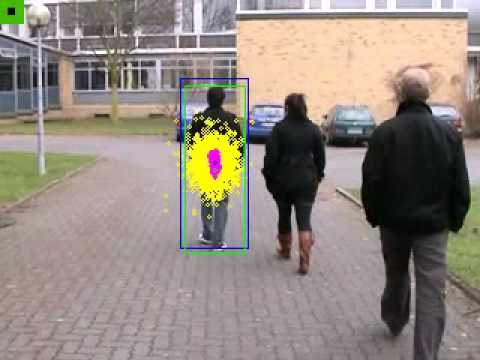
\includegraphics[width=0.32\linewidth]{Figures/particle_filter1.jpg}
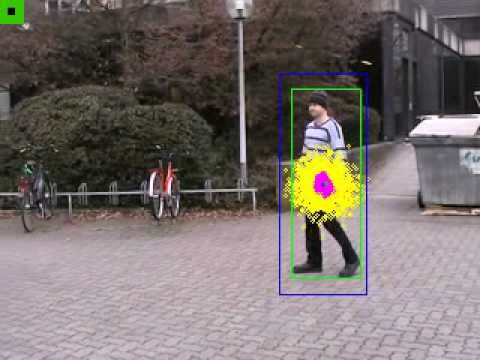
\includegraphics[width=0.32\linewidth]{Figures/particle_filter2.jpg}
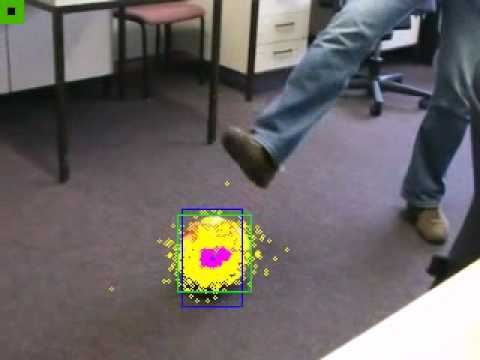
\includegraphics[width=0.32\linewidth]{Figures/particle_filter3.jpg}
}
\caption{\cite{Rittscher2000}}
\end{figure}


\subsection{Kernel Tracking}

In this type of tracking, object motion is computed using representations of a primitive object region, from one frame to the next. These algorithms differ in terms of appearance representation (features extraction) used, the number of objects tracked, and the method used for object motion estimation. 

\textbf{Density-based tracking:} According to \cite{Cheng1995}, the object is modelled with one or more probability density functions, such as Gaussian, mixture of Gaussian, Parzen windows or histogras, that describe the probability of object appearance. Mean-shift is an approach to feature space analysis. This method shifts a data point to the average of data points in its neighborhood. Mean shift uses fixed color distribution. A similar approach is called CAMSHIFT \cite{Exner2010} that handles dynamically changing color distribution by adapting the search window size and computing color distribution in the search window.

\textbf{Template-based tracking:}  These approaches apply templates of the object to calculate appearance probability on every frame of the video sequence. The most common is \textit{Template matching} \cite{Korman2013} that searchs accross the image, a region similar to the object template, defined in previous frames. The similarity measure is calculated using normalized cross correlation. A limitation of this method is its high computational cost due to brute force search. To reduce this cost, some methods limit the object search to a neighborhood near previous position.

Instead of templates, other object representations can be used for tracking. For example, color histograms or mixture models can be computed using the appearance of pixels inside the rectangular or ellipsoidal regions. To reduce computational complexitu, the similarity between object model and the hypothesized position, is computed evaluating the ratio betweem color means between model and position. The position with highest ratio is selected as current object location.

\begin{figure}[t]
	\centering
		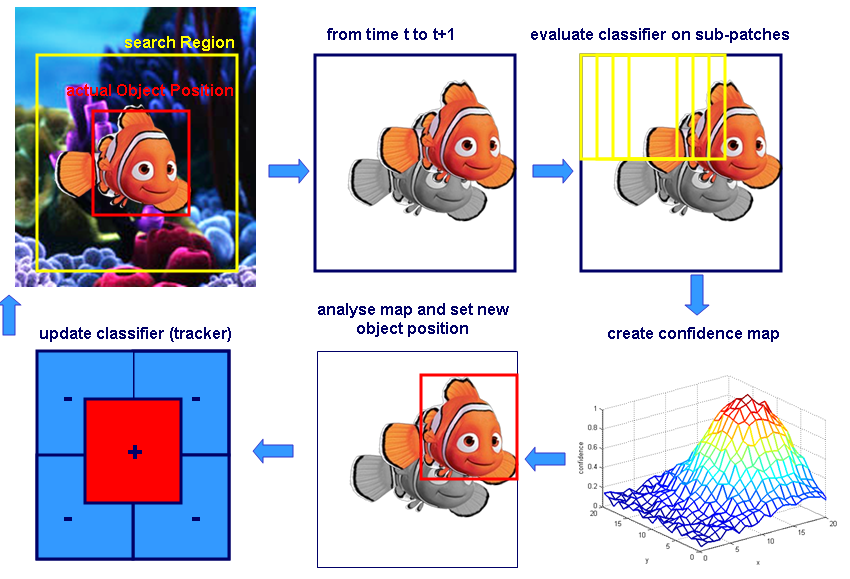
\includegraphics[width=0.7\linewidth]{Figures/overview_boost.png}
	\caption{Overview for online boosting object tracker}
	\label{fig::overview_boost}
\end{figure}	

"Tracking by detection" or "Tracking by repeated recognition" \cite{Mori2006} systems generally perform target object appearance learning. These methods are closely related to object detection (an area with great progress in computer vision) and has encouraged some successful real-time tracking algorithms \cite{Liu2007,Grabner2006}. However, many tracking algorithms employ static appearance models that are defined manually or trained at the first frame only \cite{Isard2001, Lepetit2006, Black1996, Comaniciu2000, Adam2006}, these methods are often unable to deal with significant appearance changes. This situations are difficult when there is limited knowledge of the object of interest. In order to cope this problem, an adaptive appearance model that changes during the tracking process as the appearance of the object changes, gets better results \cite{Ross2007,Matthews2004,Jepson2003}.

Boosting has been used in a wide field of machine learning tasks and applied to computer vision problems. Many tracking algorithms are based on the boosting framework \cite{Freund1997a} and is related to the work on Online Adaboost \cite{Avidan2007,Grabner2008,Oza2000}, multi-class boost \cite{Saffari2010} and MILBoost \cite{Babenko2010}. The goal of boosting is to combine many weak classifiers (usually decision stumps) into a linear strong classifier.


\subsection{Silhouette Tracking}

The object is tracked via estimation of the object region in each frame. Silhouette-based methods provide an accurate shape description for the objects that are tracked. These approaches can be divided into two main categories, shape matching and contour tracking. Shape matching \cite{Li2001} approaches search object silhouette in the current frame. Contour based, evolve initial contour to its new position in the current frame using state space models or direct minimization of some energy function \cite{Cremers2003}.

\begin{figure}[h!]
	\centering
		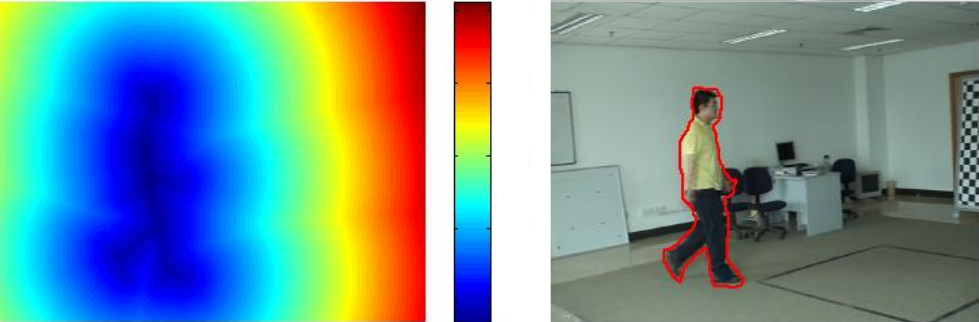
\includegraphics[width=0.9\linewidth]{Figures/contour.png}
	\caption{Illustration of an active contour representation. Left subfigure shows the signed distance map of a human contour; right image displays contour result.}
	\label{fig::contour}
\end{figure}	

\subsection{Tracking applying ensemble of trackers}

Several methods have proposed the use of ensemble classifiers within
the tracking-by-detection framework.
%The first algorithm that explicitly applies ensemble methods to
%tracking-by-detection is presented in \cite{Avidan2007}.
In this perspective, instead of ensembling the outputs of other trackers,
these methods focus on building ensemble classifiers,
such as Adaboost \cite{Avidan2007} or Bayesian probabilistic fusion \cite{Bai2013},
from weak low-level image features.
The classifier is then used to detect the target object in
new frames. Instead of working directly with low-level image features,
our ensemble tracker builds on top of tracker outputs
which are used as a more powerful mid-level representation of the target.
%Considering tracking as a binary classification problem, the author
%extends \cite{Collins2005} by using the Adaboost algorithm to
%combine a set of weak features and online updating of the object model.
%The classifier is then used to classify pixels in the next
%frames as either related to the object or background, which produces
%a confidence map of the location of the object.

Another alternative is to manually select a small set of trackers and use
prior knowledge on the behaviour of each tracker to build an ensemble.
In \cite{Santner2010a}, the authors combine a template-based tracker,
an optical flow tracker, and an online-random forest tracking-by-detection
method into a cascade.
In that case, the authors manually predefine a set of rules that decide
how to ensemble the tracker outputs. In contrast, our method can handle
a larger pool of trackers in the ensemble, since their outputs are combined
in a data-drive fashion that does not require manual rules or prior knowledge
on the behaviour of each tracker.
%The best selection is summarized into a simple
%set of rules. The authors explain that augmenting or updating in a smart way
%a simple online learner in terms of adaptivity can lead to much better results.


Sampling based approaches have also been explored for ensemble tracking.
Examples of this are the VTD \cite{Kwon2009} and
VTS \cite{Kwon2011a} trackers.
In this perspective, there is a sampling process that generates
multiple samples of target and tracker states. These trackers run in parallel
and their outputs are fused by probabilistic weighting. Therefore,
the ensemble uses a set of trackers of similiar architecture
with varying parameters. Our ensemble has the advantage of fusing outputs
of multiple trackers with no assumptions on their architectural similarity
and can leverage strenghts that different tracker architectures can provide.
%In these articles, the approaches obtain several samples of target and trackers
%states during sampling process using a Markov Chain Monte Carlo method.
%The trackers are sampled by proposing appearance models, motion models,
%state representation types, and observation types.
%Then, the sampled trackers run in parallel and interact with each other,
%covering target variations.

%The authors in \cite{Bai2013} proposed a classifier ensemble framework that
%uses Bayesian estimation theory to estimate the non-stationary distribution
%of sampled classifiers.
%In contrast with general tracking-by-detection classifiers,
%the weight vector that combines the classifiers is treated as a random
%variable and the posterior distribution of this vector is treated using
%Bayes' theory.
%Our approach presents a self-learning algorithm that enables
%object model updates based on tracking results and not from Bayesian updates of
%the classifier.

Finally, one can consider the case of offline fusion of trackers, such as in
\cite{Bailer2014}, where all trackers are applied to the entire sequence
and the ensemble is performed after the entire sequence is processed.
However, we are interested in the case of online tracking,
where the full sequence is not available beforehand. Furthermore, our online
approach is capable of steering and reinitializing failed trackers, increasing
the chances of better long-term tracking performance.

%the authors present an approach
%that merges the result of different tracking algorithms to produce a better
%tracking result.
%Based on the idea of attraction fields, which means the closer
%a fusion candidate is to a tracking result box,
%the stronger it is attracted by it.
%The result that maximizes the attraction of all trackers is chosen as a
%global result. In contrast, our fusion approach does not drop out bad tracking
%results. Our method is able to find and reinitialize outliers efficiently.
%\input{Chapters/Chapter2} 
%\input{Chapters/Chapter3}
%\input{Chapters/Chapter4} 
%\input{Chapters/Chapter5} 
%\input{Chapters/Chapter6} 
%\input{Chapters/Chapter7} 

%----------------------------------------------------------------------------------------
%	THESIS CONTENT - APPENDICES
%----------------------------------------------------------------------------------------

\addtocontents{toc}{\vspace{2em}} % Add a gap in the Contents, for aesthetics

\appendix % Cue to tell LaTeX that the following 'chapters' are Appendices

% Include the appendices of the thesis as separate files from the Appendices folder
% Uncomment the lines as you write the Appendices

%% Appendix A

\chapter{Appendix Title Here} % Main appendix title

\label{AppendixA} % For referencing this appendix elsewhere, use \ref{AppendixA}

\lhead{Appendix A. \emph{Appendix Title Here}} % This is for the header on each page - perhaps a shortened title

Write your Appendix content here.
%\input{Appendices/AppendixB}
%\input{Appendices/AppendixC}

\addtocontents{toc}{\vspace{2em}} % Add a gap in the Contents, for aesthetics

\backmatter

%----------------------------------------------------------------------------------------
%	BIBLIOGRAPHY
%----------------------------------------------------------------------------------------

\label{Bibliography}

\lhead{\emph{Bibliography}} % Change the page header to say "Bibliography"

\bibliographystyle{unsrtnatNEW} % Use the "unsrtnat" BibTeX style for formatting the Bibliography

\bibliography{References/related_work} % The references (bibliography) information are stored in the file named "Bibliography.bib"

\end{document}  